\appendix

\section{完整代码}

\begin{lstlisting}[style=Python]
#!/usr/bin/python3

import numpy as np


def create_Gaussian_kernel(cutoff_frequency):
    """
        Returns a 2D Gaussian kernel using the specified filter size standard
        deviation and cutoff frequency.

        The kernel should have:
        - shape (k, k) where k = cutoff_frequency * 4 + 1
        - mean = floor(k / 2)
        - standard deviation = cutoff_frequency
        - values that sum to 1

        Args:
        - cutoff_frequency: an int controlling how much low frequency to leave in
          the image.
        Returns:
        - kernel: numpy nd-array of shape (k, k)

        HINT:
        - The 2D Gaussian kernel here can be calculated as the outer product of two
          vectors with values populated from evaluating the 1D Gaussian PDF at each
          corrdinate.
    """
    # define 1d gaussion function
    def gaussion(x, mean, std):
        return 1 / (std * np.sqrt(2 * np.pi)) * np.exp(-0.5 * ((x - mean) / std) ** 2)
    
    def create_gaussian_naive(cutoff_frequency):
        """ Naive implementation of Gaussian kernel. """
        # define kernel size
        k = cutoff_frequency * 4 + 1
        kernel = np.zeros((k, k))

        # define mean and std
        mean = k // 2
        std = cutoff_frequency
        
        # calculate kernel for each pixel
        # each pixel is multiplied by the product of 1d gaussion function of X and 1d gaussion function of Y
        # the product of two 1d gaussion function is the 2d gaussion function
        for i in range(k):
            for j in range(k):
                kernel[i, j] = gaussion(i, mean, std) * gaussion(j, mean, std)
        
        # normalize the kernel
        kernel /= np.sum(kernel)
        return kernel
    
    def create_gaussian_numpy(cutoff_frequency):
        """ Numpy implementation of Gaussian kernel. """
        # define kernel size
        k = cutoff_frequency * 4 + 1
        kernel = np.zeros((k, k))

        # define mean and std
        mean = k // 2
        std = cutoff_frequency
        
        # create 1d gaussion function
        x = np.arange(k)
        kernel_x = gaussion(x, mean, std)
        
        # create 2d gaussion function
        kernel = np.outer(kernel_x, kernel_x)
        
        # normalize the kernel
        kernel /= np.sum(kernel)
        return kernel

    # return create_gaussian_naive(cutoff_frequency)
    return create_gaussian_numpy(cutoff_frequency)


def my_imfilter(image, filter):
    """
    Apply a filter to an image. Return the filtered image.

    Args
    - image: numpy nd-array of shape (m, n, c)
    - filter: numpy nd-array of shape (k, j)
    Returns
    - filtered_image: numpy nd-array of shape (m, n, c)

    HINTS:
    - You may not use any libraries that do the work for you. Using numpy to work
    with matrices is fine and encouraged. Using OpenCV or similar to do the
    filtering for you is not allowed.
    - I encourage you to try implementing this naively first, just be aware that
    it may take an absurdly long time to run. You will need to get a function
    that takes a reasonable amount of time to run so that the TAs can verify
    your code works.
    """
    
    # naive implementation
    def my_imfilter_naive(image, filter):
        """ Naive implementation of image filter, use for loop. """
        
        def apply_filter(patch, filter):
            """
            Apply filter to a patch of image.
            Params:
            - patch: numpy nd-array of shape (K, J)
            - filter: numpy nd-array of shape (K, J)
            Returns:
            - pixel: float
            """
            pixel = 0
            # for each pixel
            for k in range(K):
                for j in range(J):
                    # multiply the pixel value with the filter value
                    pixel += patch[k, j] * filter[k, j]
            # the final pixel value is the sum of all the pixel value multiplied by the filter value
            return pixel
        
        M, N, C = image.shape
        K, J = filter.shape

        # padding image
        # (M, N, C) -> (M + 2 * P, N + 2 * P, C)
        pad_M, pad_N = K // 2, J // 2
        image_pad = np.zeros((M + 2 * pad_M, N + 2 * pad_N, C))
        image_pad[pad_M: M + pad_M, pad_N: N + pad_N, :] = image

        image_new = np.zeros((M, N, C))
        
        # for each pixel, ignore the boundary
        for m in range(M):
            for n in range(N):
                # for each channel
                for c in range(C):
                    # get image patch by using the current pixel (i, j) as the center
                    patch = image_pad[m: m + K, n: n + J, c]
                    image_new[m, n, c] = apply_filter(patch, filter)
        
        return image_new
    
    # ===================================

    # numpy implementation, using matrix multiplication to accelerate the process
    def my_imfilter_numpy(image, filter):
        """ Numpy implementation of image filter, use matrix multiplication. """

        M, N, C = image.shape
        K, J = filter.shape
        
        # padding image
        # (M, N, C) -> (M + 2 * P, N + 2 * P, C)
        pad_M, pad_N = K // 2, J // 2
        image_pad = np.pad(image, ((pad_M, pad_M), (pad_N, pad_N), (0, 0)), 'constant')

        # image to column
        # (M, N, C) -> (M * N * C, K * j)
        image_col = np.zeros((M * N * C, K * J))
        col_idx = 0
        for m in range(M):
            for n in range(N):
                for c in range(C):
                    patch = image_pad[m: m + K, n: n + J, c]
                    image_col[col_idx] = patch.flatten()
                    col_idx += 1
        
        # apply filter
        # (M * N * C, K * J) @ (K * J, 1) -> (M * N * C, 1)
        filter_col = filter.flatten()
        image_new_col = np.dot(image_col, filter_col)
        
        # reshape the image
        image_new = image_new_col.reshape((M, N, C))
        return image_new

    # ===================================

    # numpy implementation, using stride trick to accelerate image to column
    def my_imfilter_numpy_stride_trick(image, filter):
        """ Numpy implementation of image filter, use matrix multiplication. """

        M, N, C = image.shape
        K, J = filter.shape
        
        # padding image
        # (M, N, C) -> (M + 2 * P, N + 2 * P, C)
        pad_M, pad_N = K // 2, J // 2
        image_pad = np.pad(image, ((pad_M, pad_M), (pad_N, pad_N), (0, 0)), 'constant')
        image_col = np.lib.stride_tricks.sliding_window_view(image_pad, (K, J, 1)).reshape((M * N * C, K * J))
            
        # apply filter
        # (M * N * C, K * J) @ (K * J, 1) -> (M * N * C, 1)
        filter_col = filter.flatten()
        image_new_col = np.dot(image_col, filter_col)
        
        # reshape the image
        image_new = image_new_col.reshape((M, N, C))
        return image_new

    # ===================================
    
    # fft implementation, faster but may have some error
    def my_imfilter_fft(image, filter):
        """ FFT implementation of image filter. """

        freq_filter = np.fft.fft2(filter, s=image.shape[:2])

        for c in range(image.shape[2]):
            freq_per_channel = np.fft.fft2(image[:, :, c])
            image[:, :, c] = np.fft.ifft2(freq_per_channel * freq_filter).real
    
        return image
    
    # return my_imfilter_naive(image, filter)
    # return my_imfilter_numpy(image, filter)
    return my_imfilter_numpy_stride_trick(image, filter)
    # return my_imfilter_fft(image, filter)


def create_hybrid_image(image1, image2, filter):
    """
    Takes two images and a low-pass filter and creates a hybrid image. Returns
    the low frequency content of image1, the high frequency content of image 2,
    and the hybrid image.

    Args
    - image1: numpy nd-array of dim (m, n, c)
    - image2: numpy nd-array of dim (m, n, c)
    - filter: numpy nd-array of dim (x, y)
    Returns
    - low_frequencies: numpy nd-array of shape (m, n, c)
    - high_frequencies: numpy nd-array of shape (m, n, c)
    - hybrid_image: numpy nd-array of shape (m, n, c)

    HINTS:
    - You will use your my_imfilter function in this function.
    - You can get just the high frequency content of an image by removing its low
      frequency content. Think about how to do this in mathematical terms.
    - Don't forget to make sure the pixel values of the hybrid image are between
      0 and 1. This is known as 'clipping'.
    - If you want to use images with different dimensions, you should resize them
      in the notebook code.
    """
    if image1.shape != image2.shape:
        # resize the larger image to the size of the smaller image using numpy
        image1_size = image1.shape[0] * image1.shape[1]
        image2_size = image2.shape[0] * image2.shape[1]
        if image1_size < image2_size:
            np.resize(image2, image1.shape)
        else:
            np.resize(image1, image2.shape)
    
    # get low pass by using the filter
    low_pass_image1 = my_imfilter(image1, filter)
    # get high pass by subtracting the low pass from the original image
    high_pass_image2 = image2 - my_imfilter(image2, filter)
    # hybrid image is the sum of low pass and high pass
    hybrid_image = low_pass_image1 + high_pass_image2
    
    # clip the pixel values
    hybrid_image = np.clip(hybrid_image, 0.0, 1.0)
    
    return low_pass_image1, high_pass_image2, hybrid_image

\end{lstlisting}

\newpage

\section{基于FFT的图像混合}

图\ref{fig:jupyter_output_fft}展示了基于FFT的图像混合的输出结果。可以看出,FFT难以保留图像的细节,导致混合图像的效果不如直接使用滤波器的方法。

\begin{figure}[htbp]
    \centering
    \subfloat[原始图像]{\includegraphics[width=0.2\textwidth]{images/data/1a_dog.bmp}}
    \subfloat[原始图像]{\includegraphics[width=0.2\textwidth]{images/data/1b_cat.bmp}}
    \subfloat[高斯滤波器]{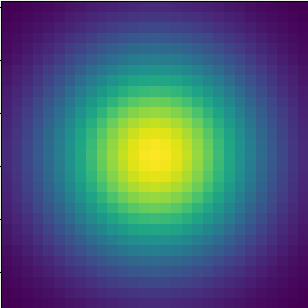
\includegraphics[width=0.2\textwidth]{images/gaussian.png}}
    \subfloat[低通图像]{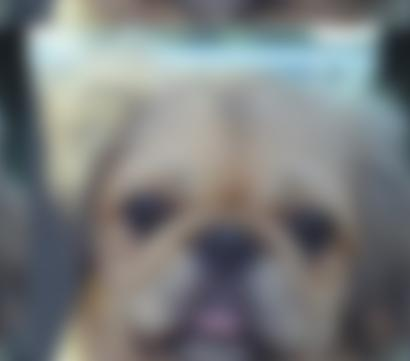
\includegraphics[width=0.2\textwidth]{images/part1_fft/low_frequencies.jpg}}
    \subfloat[高通图像]{
\includegraphics[width=0.2\textwidth]{images/part1_fft/high_frequencies.jpg}}
    \\
    \subfloat[混合图像]{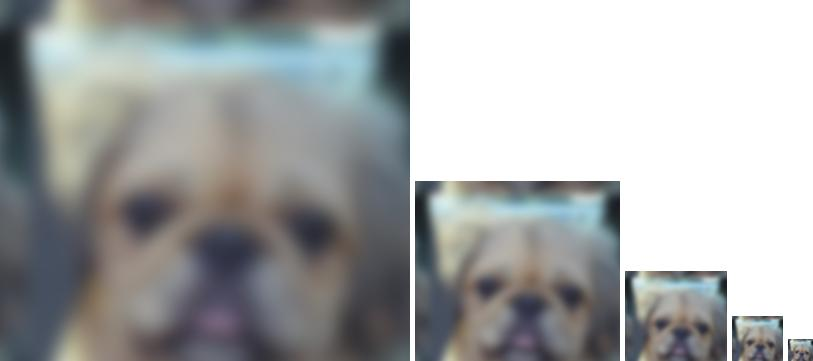
\includegraphics[width=\textwidth]{images/part1_fft/hybrid_image_scales.jpg}}
    \caption{测试程序的输出结果}
    \label{fig:jupyter_output_fft}
\end{figure}

